\chapter{Overview of Uintah} \label{Sec:Overview} 

\section{The Center for the Simulation of Accidental Fires and Explosions (C-SAFE)}

\subsection{Center History}

The Uintah software suite was created by the Center for the Simulation
of Accidental Fires and Explosions (C-SAFE).  C-SAFE was originally
created at the University of Utah in 1997 by the Department of
Energy's Accelerated Strategic Computing Initiative's (ASCI) Academic
Strategic Alliance Program (ASAP).  (ASCI has since been renamed to
the Advanced Simulation and Computing (ASC) program.)

\subsubsection{Center Objective}

C-SAFE's primary objective has been to provide a software system in
which fundamental chemistry and engineering physics are fully coupled
with nonlinear solvers, visualization, and experimental data
verification, thereby integrating expertise from a wide variety of
disciplines. Simulations using the Uintah software can help to better
evaluate the risks and safety issues associated with fires and
explosions in accidents involving both hydrocarbon and energetic
materials.

\subsubsection{Target Simulation}


The Uintah software system was designed to support the solution of a
wide range of highly dynamic physical processes using a large number
of processors.  However, our specific target simulation has been the
heating of an explosive device placed in a large hydrocarbon pool fire
and the subsequent deflagration explosion and blast wave
(Figure~\ref{Fig:fire-container-explosion}). The explosive device is a
small cylindrical steel container (4'' outside diameter) filled with
plastic bonded explosive (PBX-9501). Convective and radiative heat
fluxes from the fire heat the outside of the container and
subsequently the PBX. After some amount of time the critical
temperature in the PBX is reached and the explosive begins to rapidly
decompose into a gas. The solid$\rightarrow$gas reaction pressurizes the interior
of the steel container causing the shell to rapidly expand and
eventually rupture. The gaseous products of reaction form a blast wave
that expands outward along with pieces of the container and any
unreacted PBX. The physical processes in this simulation have a wide
range in time and length scales from microseconds and microns to
minutes and meters.  Uintah was designed as a general-purpose
fluid-structure interaction code that can simulate not only this
scenario but a wide range of related problems.

%\begin{figure}
\begin{wrapfigure}{r}{100mm}
  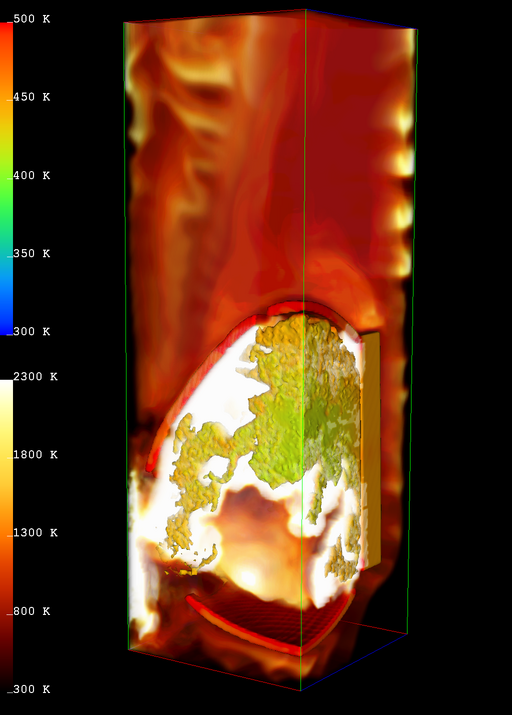
\includegraphics[scale=0.5]{fire-container-explosion-scirun.png}
  \caption{Target Simulation - Fire-Container-Explosion.}
  \label{Fig:fire-container-explosion}
\end{wrapfigure}
%\end{figure}


Complex simulations such as this require both immense computational
power and complex software. Typical simulations include solvers for
structural mechanics, fluids, chemical reactions, and material
models. All of these aspects must be integrated in an efficient manner
to achieve the scalability required to perform these simulations. The
heart of Uintah is a sophisticated computational framework that can
integrate multiple simulation components, analyze the dependencies and
communication patterns between them, and efficiently execute the
resulting multi-physics simulation.  Uintah also provides mechanisms
for automating load-balancing, checkpoint/restart, and parallel
I/O. The Uintah core was designed to be general, and is appropriate
for use in a wide range of PDE algorithms based on structured
(adaptive) grids and particle-in-cell algorithms.


\section{Uintah Software}

The Uintah Computational Framework (also referred to as Uintah or the UCF)
consists of a set of software components and libraries that facilitate
the solution of Partial Differential Equations (PDEs) on Structured
AMR (SAMR) grids using up to hundreds to thousands of processors.

One of the challenges in designing a parallel, component-based and
multi-physics application is determining how to efficiently decompose
the problem domain. Components, by definition, make local
decisions. Yet parallel efficiency is only obtained through a globally
optimal domain decomposition and scheduling of computational
tasks. Typical techniques include allocating disjoint sets of
processing resources to each component, or defining a single domain
decomposition that is a compromise between the ideal load balance of
multiple components. However, neither of these techniques will achieve
maximum efficiency for complex multi-physics problems.

Uintah uses a non-traditional approach to achieving parallelism by
employing an abstract task graph representation to describe
computation and communication. The task graph is an explicit
representation of the computation and communication that occur in the
coarse of a single iteration of the simulation (typically a timestep
or nonlinear solver iteration). Uintah components delegate decisions
about parallelism to a scheduler component by using variable
dependencies to describe communication patterns and characterizing
computational workloads to facilitate a global resource
optimization. The task graph representation has a number of
advantages, including efficient fine-grained coupling of multi-physics
components, flexible load balancing mechanisms and a separation of
application concerns from parallelism concerns. However, it creates a
challenge for scalability which we overcome by creating an implicit
definition of this graph and representing it in a distributed fashion.

%\begin{figure}
%  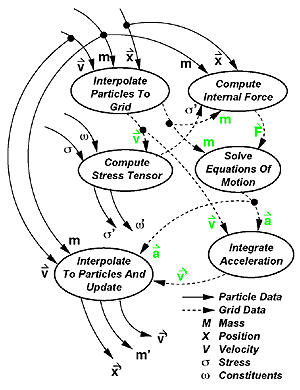
\includegraphics[scale=1]{Taskgraph-diagram.png}
%  \caption{Example Task Graph}
%  \label{fig:TaskGraph}
%\end{figure}

The primary advantage of a component-based approach is that it
facilitates the separate development of simulation algorithms, models,
and infrastructure. Components of the simulation can evolve
independently. The component-based architecture allows pieces of the
system to be implemented in a rudimentary form at first and then
evolve as the technologies mature. Most importantly, Uintah allows the
aspects of parallelism (schedulers, load-balancers, parallel
input/output, and so forth) to evolve independently of the simulation
components. Furthermore, components enable replacement of computation
pieces without complex decision logic in the code itself.

Please see the Developers Guide
(\url{http://www.uintah.utah.edu/trac/chrome/site/UintahAPI.pdf}) for more
information about the internal architecture of Uintah.

\subsection{Software Ports}

Uintah has been ported and runs well on a number of operating
systems.  These include Linux, Mac OSX, Windows, AIX, and HPuX. Simulating
small problems is perfectly feasible on 2-4 processor desktops, while
larger problems will need 100s to 1000s of processors on large
computer clusters. 

\subsection{Uintah Software History}

The UCF was orginally built on top of the SCIRun Problem Solving
Environment.  SCIRun provided a core set of software building blocks,
as well as a powerful visualization package.  While Uintah continues
to use the SCIRun core libraries, Uintah's use of the SCIRun PSE has
been retired in favor of using the VisIt visualization package from
LLNL.

